\documentclass[twoside]{book}

% Packages required by doxygen
\usepackage{fixltx2e}
\usepackage{calc}
\usepackage{doxygen}
\usepackage[export]{adjustbox} % also loads graphicx
\usepackage{graphicx}
\usepackage[utf8]{inputenc}
\usepackage{makeidx}
\usepackage{multicol}
\usepackage{multirow}
\PassOptionsToPackage{warn}{textcomp}
\usepackage{textcomp}
\usepackage[nointegrals]{wasysym}
\usepackage[table]{xcolor}

% Font selection
\usepackage[T1]{fontenc}
\usepackage[scaled=.90]{helvet}
\usepackage{courier}
\usepackage{amssymb}
\usepackage{sectsty}
\renewcommand{\familydefault}{\sfdefault}
\allsectionsfont{%
  \fontseries{bc}\selectfont%
  \color{darkgray}%
}
\renewcommand{\DoxyLabelFont}{%
  \fontseries{bc}\selectfont%
  \color{darkgray}%
}
\newcommand{\+}{\discretionary{\mbox{\scriptsize$\hookleftarrow$}}{}{}}

% Page & text layout
\usepackage{geometry}
\geometry{%
  a4paper,%
  top=2.5cm,%
  bottom=2.5cm,%
  left=2.5cm,%
  right=2.5cm%
}
\tolerance=750
\hfuzz=15pt
\hbadness=750
\setlength{\emergencystretch}{15pt}
\setlength{\parindent}{0cm}
\setlength{\parskip}{3ex plus 2ex minus 2ex}
\makeatletter
\renewcommand{\paragraph}{%
  \@startsection{paragraph}{4}{0ex}{-1.0ex}{1.0ex}{%
    \normalfont\normalsize\bfseries\SS@parafont%
  }%
}
\renewcommand{\subparagraph}{%
  \@startsection{subparagraph}{5}{0ex}{-1.0ex}{1.0ex}{%
    \normalfont\normalsize\bfseries\SS@subparafont%
  }%
}
\makeatother

% Headers & footers
\usepackage{fancyhdr}
\pagestyle{fancyplain}
\fancyhead[LE]{\fancyplain{}{\bfseries\thepage}}
\fancyhead[CE]{\fancyplain{}{}}
\fancyhead[RE]{\fancyplain{}{\bfseries\leftmark}}
\fancyhead[LO]{\fancyplain{}{\bfseries\rightmark}}
\fancyhead[CO]{\fancyplain{}{}}
\fancyhead[RO]{\fancyplain{}{\bfseries\thepage}}
\fancyfoot[LE]{\fancyplain{}{}}
\fancyfoot[CE]{\fancyplain{}{}}
\fancyfoot[RE]{\fancyplain{}{\bfseries\scriptsize Generated by Doxygen }}
\fancyfoot[LO]{\fancyplain{}{\bfseries\scriptsize Generated by Doxygen }}
\fancyfoot[CO]{\fancyplain{}{}}
\fancyfoot[RO]{\fancyplain{}{}}
\renewcommand{\footrulewidth}{0.4pt}
\renewcommand{\chaptermark}[1]{%
  \markboth{#1}{}%
}
\renewcommand{\sectionmark}[1]{%
  \markright{\thesection\ #1}%
}

% Indices & bibliography
\usepackage{natbib}
\usepackage[titles]{tocloft}
\setcounter{tocdepth}{3}
\setcounter{secnumdepth}{5}
\makeindex

% Hyperlinks (required, but should be loaded last)
\usepackage{ifpdf}
\ifpdf
  \usepackage[pdftex,pagebackref=true]{hyperref}
\else
  \usepackage[ps2pdf,pagebackref=true]{hyperref}
\fi
\hypersetup{%
  colorlinks=true,%
  linkcolor=blue,%
  citecolor=blue,%
  unicode%
}

% Custom commands
\newcommand{\clearemptydoublepage}{%
  \newpage{\pagestyle{empty}\cleardoublepage}%
}

\usepackage{caption}
\captionsetup{labelsep=space,justification=centering,font={bf},singlelinecheck=off,skip=4pt,position=top}

%===== C O N T E N T S =====

\begin{document}

% Titlepage & ToC
\hypersetup{pageanchor=false,
             bookmarksnumbered=true,
             pdfencoding=unicode
            }
\pagenumbering{roman}
\begin{titlepage}
\vspace*{7cm}
\begin{center}%
{\Large Teste \\[1ex]\large 1.\+0 }\\
\vspace*{1cm}
{\large Generated by Doxygen 1.8.11}\\
\end{center}
\end{titlepage}
\clearemptydoublepage
\tableofcontents
\clearemptydoublepage
\pagenumbering{arabic}
\hypersetup{pageanchor=true}

%--- Begin generated contents ---
\chapter{File Index}
\section{File List}
Here is a list of all files with brief descriptions\+:\begin{DoxyCompactList}
\item\contentsline{section}{src/\hyperlink{calcula_8cpp}{calcula.\+cpp} }{\pageref{calcula_8cpp}}{}
\item\contentsline{section}{src/\hyperlink{main_8cpp}{main.\+cpp} }{\pageref{main_8cpp}}{}
\item\contentsline{section}{src/\hyperlink{mostra_8cpp}{mostra.\+cpp} }{\pageref{mostra_8cpp}}{}
\end{DoxyCompactList}

\chapter{File Documentation}
\hypertarget{calcula_8cpp}{}\section{src/calcula.cpp File Reference}
\label{calcula_8cpp}\index{src/calcula.\+cpp@{src/calcula.\+cpp}}
{\ttfamily \#include \char`\"{}calcula.\+h\char`\"{}}\\*
Include dependency graph for calcula.\+cpp\+:
\nopagebreak
\begin{figure}[H]
\begin{center}
\leavevmode
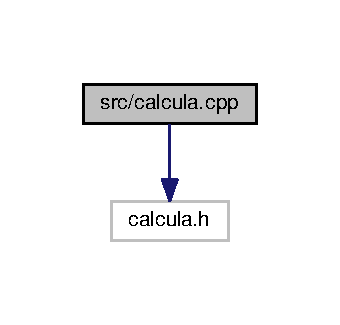
\includegraphics[width=163pt]{calcula_8cpp__incl}
\end{center}
\end{figure}
\subsection*{Functions}
\begin{DoxyCompactItemize}
\item 
int \hyperlink{calcula_8cpp_a8f4955ac9731a6239fafcfc505c9f404}{fatorial} (int $\ast$val)
\begin{DoxyCompactList}\small\item\em Funcao recursiva que calcula o fatorial de um numero. \end{DoxyCompactList}\item 
int \hyperlink{calcula_8cpp_ae68ebc37bafc99b6e3ef240f1554d2e0}{primo} (int $\ast$result\+Fat, int $\ast$chk)
\begin{DoxyCompactList}\small\item\em Funcao recursiva que avalia qual o numero anterior ao resultado do fatorial é o primo mais proximo. \end{DoxyCompactList}\end{DoxyCompactItemize}


\subsection{Function Documentation}
\index{calcula.\+cpp@{calcula.\+cpp}!fatorial@{fatorial}}
\index{fatorial@{fatorial}!calcula.\+cpp@{calcula.\+cpp}}
\subsubsection[{\texorpdfstring{fatorial(int $\ast$val)}{fatorial(int *val)}}]{\setlength{\rightskip}{0pt plus 5cm}int fatorial (
\begin{DoxyParamCaption}
\item[{int $\ast$}]{val}
\end{DoxyParamCaption}
)}\hypertarget{calcula_8cpp_a8f4955ac9731a6239fafcfc505c9f404}{}\label{calcula_8cpp_a8f4955ac9731a6239fafcfc505c9f404}


Funcao recursiva que calcula o fatorial de um numero. 


\begin{DoxyParams}{Parameters}
{\em $\ast$val} & ponteiro que aponta para o valor passado pelo usuario \\
\hline
\end{DoxyParams}
\begin{DoxyReturn}{Returns}
valor do fatorial do numero informado pelo usuario 
\end{DoxyReturn}

\begin{DoxyCode}
8                        \{
9     \textcolor{keywordflow}{if}(*val == 1 || *val == 0) \{
10         \textcolor{keywordflow}{return} 1;
11     \} \textcolor{keywordflow}{else} \{
12         \textcolor{keywordtype}{int} anterior = *val - 1;\textcolor{comment}{//armazena o valor inteiro anterior a *val}
13         \textcolor{keywordflow}{return} *val * \hyperlink{calcula_8cpp_a8f4955ac9731a6239fafcfc505c9f404}{fatorial}(&anterior);
14     \}
15 \}
\end{DoxyCode}
\index{calcula.\+cpp@{calcula.\+cpp}!primo@{primo}}
\index{primo@{primo}!calcula.\+cpp@{calcula.\+cpp}}
\subsubsection[{\texorpdfstring{primo(int $\ast$result\+Fat, int $\ast$chk)}{primo(int *resultFat, int *chk)}}]{\setlength{\rightskip}{0pt plus 5cm}int primo (
\begin{DoxyParamCaption}
\item[{int $\ast$}]{result\+Fat, }
\item[{int $\ast$}]{chk}
\end{DoxyParamCaption}
)}\hypertarget{calcula_8cpp_ae68ebc37bafc99b6e3ef240f1554d2e0}{}\label{calcula_8cpp_ae68ebc37bafc99b6e3ef240f1554d2e0}


Funcao recursiva que avalia qual o numero anterior ao resultado do fatorial é o primo mais proximo. 


\begin{DoxyParams}{Parameters}
{\em $\ast$result\+Fat} & ponteiro que aponta para o resultado do calculo do fatorial \\
\hline
{\em $\ast$chk} & paramatro de avaliacao para determinar se um numero é primo \\
\hline
\end{DoxyParams}
\begin{DoxyReturn}{Returns}
numero primo mais proximo do valor apontado por $\ast$result\+Fat 
\end{DoxyReturn}

\begin{DoxyCode}
23                                     \{
24     \textcolor{keywordflow}{if}(*chk == 1) \{
25         \textcolor{keywordflow}{return} *resultFat;
26     \} \textcolor{keywordflow}{else} \{
27         \textcolor{keywordflow}{if}(*resultFat%*chk == 0) \{
28             *resultFat -= 1;
29             *chk = *resultFat/2;
30             \textcolor{keywordflow}{return} \hyperlink{calcula_8cpp_ae68ebc37bafc99b6e3ef240f1554d2e0}{primo}(resultFat, chk);
31         \} \textcolor{keywordflow}{else} \{
32             *chk -= 1;
33             \textcolor{keywordflow}{return} \hyperlink{calcula_8cpp_ae68ebc37bafc99b6e3ef240f1554d2e0}{primo}(resultFat, chk);
34         \}
35     \}
36 \}\end{DoxyCode}

\hypertarget{main_8cpp}{}\section{src/main.cpp File Reference}
\label{main_8cpp}\index{src/main.\+cpp@{src/main.\+cpp}}
{\ttfamily \#include $<$iostream$>$}\\*
{\ttfamily \#include $<$cstdlib$>$}\\*
{\ttfamily \#include \char`\"{}calcula.\+h\char`\"{}}\\*
{\ttfamily \#include \char`\"{}mostra.\+h\char`\"{}}\\*
Include dependency graph for main.\+cpp\+:
\nopagebreak
\begin{figure}[H]
\begin{center}
\leavevmode
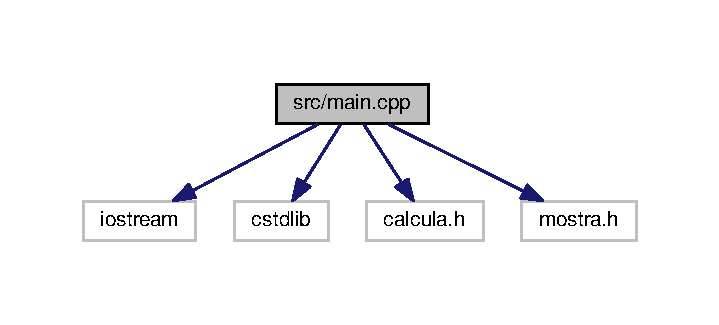
\includegraphics[width=345pt]{main_8cpp__incl}
\end{center}
\end{figure}
\subsection*{Functions}
\begin{DoxyCompactItemize}
\item 
int \hyperlink{main_8cpp_a0ddf1224851353fc92bfbff6f499fa97}{main} (int argc, char $\ast$argv\mbox{[}$\,$\mbox{]})
\begin{DoxyCompactList}\small\item\em Funcao principal. \end{DoxyCompactList}\end{DoxyCompactItemize}


\subsection{Function Documentation}
\index{main.\+cpp@{main.\+cpp}!main@{main}}
\index{main@{main}!main.\+cpp@{main.\+cpp}}
\subsubsection[{\texorpdfstring{main(int argc, char $\ast$argv[])}{main(int argc, char *argv[])}}]{\setlength{\rightskip}{0pt plus 5cm}int main (
\begin{DoxyParamCaption}
\item[{int}]{argc, }
\item[{char $\ast$}]{argv\mbox{[}$\,$\mbox{]}}
\end{DoxyParamCaption}
)}\hypertarget{main_8cpp_a0ddf1224851353fc92bfbff6f499fa97}{}\label{main_8cpp_a0ddf1224851353fc92bfbff6f499fa97}


Funcao principal. 


\begin{DoxyCode}
11                                  \{
12 
13     \textcolor{keywordtype}{int} valor = atoi(argv[1]);\textcolor{comment}{//armazena valor inteiro passado pelo usuario em linha de comando}
14     \textcolor{keywordtype}{int} valorInicial = valor; \textcolor{comment}{//armazena valor para salvar seu valor original}
15     \textcolor{keywordtype}{int} resultadoFatorial = \hyperlink{calcula_8cpp_a8f4955ac9731a6239fafcfc505c9f404}{fatorial}(&valor);
16     \textcolor{keywordtype}{int} check = resultadoFatorial/2;
17     \textcolor{keywordtype}{int} resultadoPrimo = \hyperlink{calcula_8cpp_ae68ebc37bafc99b6e3ef240f1554d2e0}{primo}(&resultadoFatorial, &check);
18     \hyperlink{mostra_8cpp_a385bafcdbda785303563990b110f86af}{mostra}(&valorInicial, &resultadoPrimo);
19 
20     \textcolor{keywordflow}{return} 0;
21 \}\end{DoxyCode}

\hypertarget{mostra_8cpp}{}\section{src/mostra.cpp File Reference}
\label{mostra_8cpp}\index{src/mostra.\+cpp@{src/mostra.\+cpp}}
{\ttfamily \#include $<$iostream$>$}\\*
{\ttfamily \#include \char`\"{}mostra.\+h\char`\"{}}\\*
Include dependency graph for mostra.\+cpp\+:
\nopagebreak
\begin{figure}[H]
\begin{center}
\leavevmode
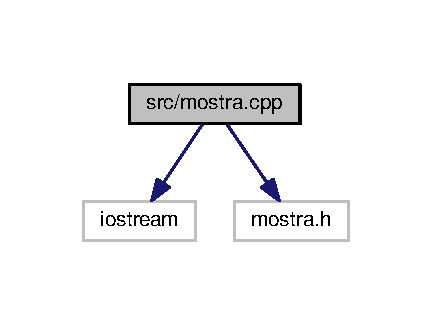
\includegraphics[width=207pt]{mostra_8cpp__incl}
\end{center}
\end{figure}
\subsection*{Functions}
\begin{DoxyCompactItemize}
\item 
void \hyperlink{mostra_8cpp_a385bafcdbda785303563990b110f86af}{mostra} (int $\ast$val\+Inic, int $\ast$result\+Prim)
\end{DoxyCompactItemize}


\subsection{Function Documentation}
\index{mostra.\+cpp@{mostra.\+cpp}!mostra@{mostra}}
\index{mostra@{mostra}!mostra.\+cpp@{mostra.\+cpp}}
\subsubsection[{\texorpdfstring{mostra(int $\ast$val\+Inic, int $\ast$result\+Prim)}{mostra(int *valInic, int *resultPrim)}}]{\setlength{\rightskip}{0pt plus 5cm}void mostra (
\begin{DoxyParamCaption}
\item[{int $\ast$}]{val\+Inic, }
\item[{int $\ast$}]{result\+Prim}
\end{DoxyParamCaption}
)}\hypertarget{mostra_8cpp_a385bafcdbda785303563990b110f86af}{}\label{mostra_8cpp_a385bafcdbda785303563990b110f86af}
Funcao que mostra na tela o numero primo mais proximo 
\begin{DoxyParams}{Parameters}
{\em $\ast$val\+Inic} & ponteiro que aponta para o valor origina passado pelo usuario \\
\hline
{\em $\ast$result\+Prim} & ponteiro que aponta para o numero primo mais proximo encontrado \\
\hline
\end{DoxyParams}
\begin{DoxyReturn}{Returns}
void 
\end{DoxyReturn}

\begin{DoxyCode}
11                                            \{
12     cout << \textcolor{stringliteral}{"O número primo mais próximo do fatorial de "} << *valInic << \textcolor{stringliteral}{" encontrado foi: "} << *resultPrim
       << endl;
13 \}
\end{DoxyCode}

%--- End generated contents ---

% Index
\backmatter
\newpage
\phantomsection
\clearemptydoublepage
\addcontentsline{toc}{chapter}{Index}
\printindex

\end{document}
